% 1_introduction.tex

\cleardoublepage
\chapter{Introduction}

focus on objectives and chapter outlines,
give to Kearney to review first

for thesis review - 1 page dot point with where im up to
-refer to stated objectives from mid cand
  	
  	
  	  Airbreathing engines are an ideal candidate for producing the next generation of space access
  	systems. Airbreathing engines produce higher specific impulse than rockets, and require far less propellant to be carried on-board a launch vehicle.   	 
  	The mass savings gained by using airbreathing engines allow launch vehicles to be designed to be reusable, capable of manoeuvring aerodynamically and landing similarly to a conventional aircraft. 
  	The primary engines in consideration for launch vehicles are ramjet and scramjet engines.
  	Ramjets and scramjets rely on the high velocity of the aircraft to compress the flow of air entering the engine before combustion.  Ramjets slow the air to subsonic speeds and are suited to operation at low Mach numbers, whereas scramjets keep the flow supersonic throughout, and operate within the hypersonic regime, above Mach 5. 
  	
  	

  	 
  	 
  	 The use of airbreathing engines for reusability has particular applicability to small satellite launchers, currently an area of rapid expansion in the space sector. 
  	 As the small satellite market increases, so does the demand for launchers tailored to the specific orbit and scheduling needs of each satellite. Reusability of small satellite launchers is more complex than for large launchers, as the additional systems necessary for reusability add a larger fraction of system mass, and require a proportionally larger fuel mass. 
  	 The higher efficiency and reduced propellant mass of airbreathing vehicles allows the additional mass of the systems necessary for reusability to be mitigated. An airbreathing vehicle can be designed in a similar fashion to a conventional aircraft, with wings, stabilisers and ailerons. However, a launch system cannot be solely powered by airbreathing engines, rocket power is necessary for at least the exoatmospheric portion of the trajectory. The design of the trajectory of a partially-airbreathing launch system is particularly important to its performance. 
  	   The airbreathing engines of a ramjet or scramjet-powered stage require high dynamic pressure to operate effectively, and airbreathing engines are generally designed for high lift-to-drag. Conversely, rocket-powered stages produce more thrust at higher altitude, and are generally designed for weight efficiency. For these launch systems, the various stages and engines involved during launch require trade-offs in engine efficiency and thrust generation, stage mass, and vehicle aerodynamics. These factors require the launch trajectory of the system to be thoroughly simulated and optimised, to ensure that the launch vehicle is operating effectively. 
 	  
  	  	\begin{figure}[ht]
  	  		\centering
  	  		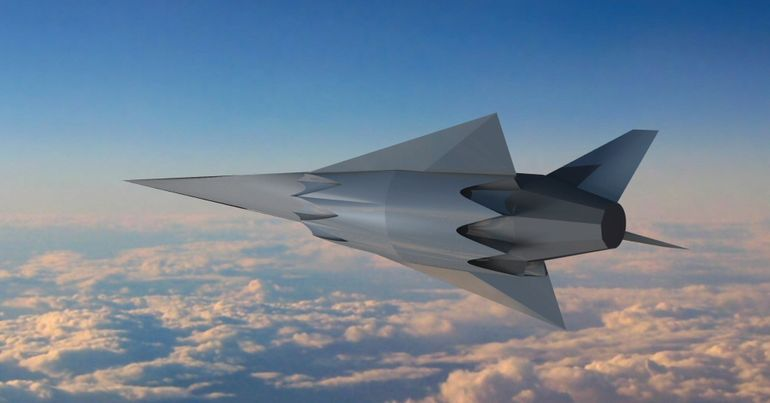
\includegraphics[width=0.7\linewidth]{figures/1_introduction/project-spartan}
  	  		\caption{The scramjet-powered second stage of the SPARTAN CITATIONXX.}
  	  		\label{fig:project-spartan}
  	  	\end{figure}
  	  	


-something about taking out predispositions int rajectory design (we dont know what it should look like, so potimal control be good)

  Calculating the optimal trajectory for a space launch system is an integral part of the preliminary vehicle and mission design process. Calculating the optimal trajectory profile for a launch system typically requires the use of optimal control theory. Optimal control theory is a general set of techniques which find a control law to maximise a given metric of a system. For a launch vehicle, optimal control allows the best possible payload-to-orbit to be calculated in simulations during design. 
Optimal control theory allows a trajectory to be calculated in which the flight path of each individual vehicle is considered simultaneously to produce a maximum-payload trajectory. 
Optimal control is particularly important for launch systems incorporating airbreathing engines, where the performance of each vehicle is thoroughly different. 
Optimal control is able to produce an optimised trajectory which satisfies equality or inequality constraints. These constraints allow for the physical limitations of the vehicle, such as heating and structural loading limits, to be imposed. These constraints also allow any necessary mission conditions to be established, such as orbital velocity and fly-back. 
  
  
  	   
  	   A three stage rocket-scramjet-rocket launch system, designated the SPARTAN, is being developed by The University of Queensland. This system is designed to be partially reusable, with the first stage rocket and second stage scramjet vehicles flying back to the initial launch site. 
  	   In previous studies it has been assumed that the optimal trajectory for the scramjet powered vehicle is at its
  	   maximum dynamic pressure and all other trajectory stages have conformed to this assumption. This study will aim to produce an optimal
  	   trajectory profile which may be applied to any rocket-airbreathing-rocket system for delivering small
  	   satellites to Earth orbit. 

  	\textcolor{red}{Add image of the final trajectory}
  \section{Research aims}

    The overall aim of this thesis is to apply state of the art numerical optimisation techniques to the trajectory of a rocket-scramjet-rocket small satellite launch system. The purpose of this optimised trajectory is to maximise the payload-to-orbit capabilities of the launch system, thereby also maximising the cost efficiency of the system. 
    
    \textcolor{red}{add more, flexibility, turn around time, operability}
    

    \noindent This will be achieved through the following objectives:
 \textcolor{red}{IJ - not objectives, redo}
    \begin{enumerate}
    	 \item \emph{}\\


\item \emph{}\\

    	
      \item \emph{}\\


      \item \emph{}\\



    \end{enumerate}

  \clearpage
  \section{Thesis outline}

    

    \subsubsection*{Chapter 2 - Literature Review}

      This chapter presents a review of literature related to the different aspects of this thesis. The theory behind scramjet propulsion is presented, followed by a background of reusable and small satellite launch systems. A review of the trajectories of partially-airbreathing launch systems is presented, comparing the optimised trajectories of various conceptual vehicles. An overview of optimal control theory is presented, with particular emphasis on the pseudospectral method of optimal control which is employed within this study. Lastly, an overview of the optimal control and aerodynamic solvers which are used in this study is presented.
      

    \subsubsection*{Chapter 3 - Launch Vehicle Baseline Design}

      This chapter provides details of the design, aerodynamics and engine models of all three stages. The SPARTAN scramjet-powered stage is presented first, followed by the first and third stages, due to the external scramjet vehicle design being taken from prior work. The design of each stage is presented, followed by the propulsion model, and finally the aerodynamic characteristics. 
      
      
      \subsubsection*{Chapter 4 - LODESTAR}
      
      This chapter details the method used for the simulation and optimisation of the trajectory, packaged within the trajectory analysis program LODESTAR, which has been created for this study. The specifics of the optimal control methodology used are presented, along with relevant examples. The simulation methodology is detailed, along with the construction of the optimal control simulation. The specific set-up of the optimal control program is detailed for each trajectory stage, specifying the costs and constraints which drive the optimal control solver. Finally, the methods for validating the final solutions are specified.
      
      \subsubsection*{Chapter 5 - Optimised Trajectory}
      
      This chapter presents the results of the trajectory optimised using LODESTAR. The ascent of the SPARTAN and third stage rocket are optimised along with the fly-back of the SPARTAN, for maximum payload-to-orbit. 
      
      \subsubsection*{Chapter 6 - Trajectory Sensitivity Study}
      
      \subsubsection*{Chapter 7 - Third Stage Sizing Study}

    \subsubsection*{Conclusions}

      The body of this thesis concludes by summarising the most significant findings from
